\chapter{SQL -- その1}\label{chap:sql-part1}

\ref{chap:relational-data-model}章まで定義の話が続いてきたので，本章からは関係データベースを扱うための実践的な話題に移りましょう．

データベースからデータを抽出したり，データベースに新しいデータを登録したりするには，データベースを操作するための具体的なツールが必要となります．
\strong{SQL（Structured Query Language）} は関係データベースの操作に特化した言語です．
SQLはISOによって国際的に標準化されています．
よく用いられる関係データベース管理システム（RDBMS）としては，MySQL\footnote{\url{https://ja.wikipedia.org/wiki/MySQL}}やPostgreSQL\footnote{\url{https://ja.wikipedia.org/wiki/PostgreSQL}}，Oracle Database\footnote{\url{https://ja.wikipedia.org/wiki/Oracle_Database}}，Microsoft SQL Server\footnote{\url{https://ja.wikipedia.org/wiki/Microsoft\_SQL\_Server}}などが挙げられますが，どのRDBMSにもSQLは実装されています．

SQLを使うことで，関係データベースのユーザは
\begin{itemize}
\item データの登録（Create）
\item データの読み出し（Read）
\item データの更新（Update）
\item データの削除（Delete）
\end{itemize}
が可能となります\footnote{データの作成，読み出し，更新，削除はデータベースに求められる主要な操作で，それぞれの頭文字を取ってCRUD（クラッド）と呼ばれる．}．
ここで，関係データベースのユーザは人間だけでなく，アプリケーションなどのプログラムであっても構いません．
例えば，データ分析者は，データベースから分析に必要となるデータを抽出する際にSQLを使っています．
また，ショッピングサイトでは，消費者がある商品の注文ボタンを押すと，ウェブアプリケーションのプログラムがSQLを通じてデータベースに注文記録を登録するということが行われています．

ところで，SQLはデータベースに対する問い合わせ言語であって，プログラミング言語ではありません．
SQLはプログラミング言語に比べて覚えることは少なく，問い合わせ内容を英語に近い形で書き下すことができるよう設計されています．
もしあなたがデータ分析人材を目指しているのであれば，ソフトウェアを開発することが目的ではありませんから，高度なプログラミング能力を持つ必要はありません．
しかし，大量のデータを活かすことが期待されている今日，関係データベースに納められた大量のデータを自由自在に扱うためには，\strong{SQLの習得は必須}です．
本章ではデータ分析の基本となる「読み出し（Read）」の基礎に絞って解説し，複雑な読み出しやレコードの登録，更新などは次章以降で説明します．


\begin{notebox}{SQLの読み方}
SQLは「エス・キュー・エル」と読む．SQLは1970年代にIBM社が開発したデータベース管理システムSystem Rの操作言語SEQUELを起源としています\cite{SEQUEL}．
関係データベースに熱狂していた世代の人の中には，SEQUELの名残でSQLのことを「シークエル」と呼ぶ人もいます．
\end{notebox}

\begin{warningbox}{SQLにも方言がある}
RDBMSによって，SQLで使用できる関数が異なったりすることがあります．
特にSQLiteについては，簡易的なRDMBSということもあり，他のRDBMSでは実装されている機能や関数が実装されていない場合があります．
自分が書いたSQL文がうまく動作しない場合は，マニュアルに当たってみてください．
\end{warningbox}


\section{SQLと関係データモデルの比較}\label{chap:sql-vs-relational-data-model}
SQLは関係データベースを操作する言語で，それが扱うデータモデルは関係データモデルを実用的に拡張したものです．
ところが，「実用」のSQLデータモデルと「理論」の関係データモデルでは，同様の概念が異なる用語で定義されていることがあります．
以下，SQLと関係データモデルの用語の比較です．

\begin{table}[h]
    \centering
    \caption{SQLと関係データモデルの用語の比較}
    \begin{tabular}{ll}
    \toprule
    \textbf{関係データモデル}             & \textbf{SQL}            \\ \midrule
    関係（リレーション; relation） & 表（テーブル; table） \\
    タプル（tuple）           & レコード or 行（row） \\
    属性（attribute）        & 列（カラム; column） \\
    定義域（ドメイン; domain）    & データ型           \\ \bottomrule
    \end{tabular}
    \label{tab:sql-vs-relational-data-model}
\end{table}

表\ref{tab:sql-vs-relational-data-model}はSQLと関係データモデルで登場する類似概念を整理していますが，これら以外に重要な違いが3つあります．
1つ目が，SQLでは同じ内容を示すレコードの存在（重複）が許されることがあるという点です．
関係データモデルにおいてSQLのレコードに相当するのがタプルですが，タプルは（数学的な）集合の要素であるため，関係データモデルでは同じ内容のタプルを重複して存在することは許されていません．
ところが，SQLでは問い合わせの結果の中では同じ内容のレコードの存在が許されています．
これは，現実の関係データベースに対する問い合わせにおいては，レコードが重複することを許可しないと都合が悪い場合があるからです．
例えば，同じカテゴリに属する商品の売り上げの平均額を計算する場合，カテゴリ名に対応する商品の売り上げ高をまず抽出する必要がありますが，仮にカテゴリAに属する商品XとYの売り上げが同じ額の場合，抽出したレコードには同じ内容のレコードが2つ含まれることになります．
このとき，もしSQLが同じ内容のレコードの重複を許さなければ，商品X，Yいずれかの売り上げ情報が消えることになり，売り上げ額の平均計算が正しく行えなくなります．

違いの2つ目は，SQLでは問い合わせ結果に対して順序関係を定義できる点です．
関係データモデルでは関係中のタプルには順序関係がありません．
タプルは集合の要素であり，集合には順序の概念がないからです．
ところが，実用的な関係データベースに対する問い合わせにおいては，問い合わせ結果のレコードに順序を定義したい場合があります．
例えば，売り上げを記録している関係があったとき，売り上げ順に関係中のタプルを並べたくなりますよね．
関係データモデルのタプルと同様，SQLにおいてもテーブル中のレコードには順序関係がありません．
しかしながら，先のようなニーズに応えるため，SQLでは問い合わせの結果得られたレコードには順序づけを行うことができます．

3つ目の違いは，\strong{NULL値}の有無です．
関係データモデルでは各属性は必ずドメインで定義された値を持ちます．
一方，現実的にはある属性の値が存在しない，あるいは未定義（不明）のケースがあり得ます．
このような状況を表現するために，SQLでは特殊な値である\strong{NULL値}（ヌルと読む）を用います．

関係データモデルとSQLの対応付けが終わりましたので，早速関係データを具体的に操作する方法を見ていきましょう．


\section{準備}
以下の説明では，SQLite\footnote{\url{https://www.sqlite.org/index.html}}と解説用に作成した仮想データを用いてSQLについて解説します．

\subsection{SQLite}
SQLiteは個人用のPCでも簡単に利用できる，軽量なRDBMSです．
SQLiteは軽量であるものの，SQLの基本的な機能については十分にサポートされているため，SQLの学習に適しています．

SQLiteを利用する最も簡単な方法は，DB Browser for SQLiteを利用することです．
DB Browser for SQLiteの公式サイト（\url{https://sqlitebrowser.org/}）にはWindows，macOS，Linux向けのインストーラが配布されているので，本書で説明するSQLを実際に実行してみたい方はダウンロードしてください．

\subsection{仮想データ}
本章では，SQL解説用に著者が作成した仮想データを用います．
用意した仮想データは，こちらのURL（\url{https://github.com/trycycle/database-textbook/xxxx}）よりダウンロードできます．
ダウンロードしたファイル\graybox{sql1-example.db}はSQLiteのデータベースファイルです．
DB Browser for SQLiteなどのSQLiteクライアントソフトを用いて，本章用の関係データベースを操作することができます．

ダウンロードしたデータは，1章で取り上げたような小売店ショッピングサイトに掲載された商品の情報を管理する関係データベースです．
この関係データベースには，表\ref{table:product-table}のように，商品ID，商品名，カテゴリ，メーカー，価格，在庫数を列（属性）として持つ「商品」テーブルが格納されています．
以後，このテーブルが格納された関係データベースが手元にあると想定して，SQLの使い方を説明します．
\begin{table}[h]
    \centering
    \caption{「商品」テーブル}
    \scalebox{0.93}{
    \begin{tabular}{@{}llllll@{}}
    \toprule
    \textbf{商品ID} & \textbf{商品名} & \textbf{カテゴリ} & \textbf{メーカー} & \textbf{価格} & \textbf{在庫数} \\ \midrule
    P001 & 国産カレーパン         & パン     & A製パン       & 270 & 206 \\
    P002 & 職人仕込みクロワッサン & パン     & Bフーズ & 230 & 443 \\
    P003 & 国産チキンカレー       & レトルト & C食品     & 420 & 149 \\
    P004 & 天然中華丼の素         & レトルト & Dフード       & 180 & 166 \\
    P005 & 味わい焼肉のたれ       & 調味料   & E食品         & 890 & 18  \\
         &                        & $\vdots$ &                  &     &      \\
    P500 & 辛口めんつゆ          & 調味料 & E食品 & 590 & 19 \\ \bottomrule
    \end{tabular}
    }
    \label{tab:product-table}
\end{table}


\section{SQLの基本形}
関係データベースに対する最も典型的な問い合わせ要求は，
\begin{itemize}
\item 特定の\strong{表（table，テーブル）}から
\item \strong{列（column，カラム）} が特定の条件を満たす\strong{行（row）}\footnote{レコード（record）と呼ぶこともある．} を見つけ出し
\item 結果を表形式で出力する
\end{itemize}
というものです．
問い合わせのために記述するSQL文のことを\strong{クエリ（query）} と呼びます．

SQLによる代表的なクエリは，コード\ref{code:first-sql}に記したようなの形式の\strong{SELECT文}です．
\begin{figure}[h]
    \begin{minted}[gobble=1,
        bgcolor=background,
        fontsize=\small,
        linenos=false,
        xleftmargin=0em]{sql}

    SELECT
        商品名
    FROM
        商品
    WHERE
        在庫数 >= 100;

    \end{minted}
    \captionsetup{name=コード}
    \caption{単純なSELECT文}
    \label{code:first-sql}
\end{figure}
このクエリは，
\begin{framed}
「商品」テーブルから「在庫数」という列の値が100以上である行を見つけ，その行の列「商品名」を出力してください
\end{framed}
という問い合わせ要求を表現したものです．
これら要求を表現するために，コード\ref{code:first-sql}のクエリでは
\begin{itemize}
\item \graybox{SELECT}句を用いて「問い合わせ結果に表示したい列情報」，
\item \graybox{FROM}句を用いて「参照したい表」，
\item \graybox{WHERE}句を用いて「表示する際の条件」
\end{itemize}
を指定しています．
上記要求を英語に直してみると，SQL文は問い合わせ要求をできるだけ直感的に表現しようとしていることが見て取れます．

コード\ref{code:first-sql}のクエリは単純な例に過ぎませんが，関係データベースからデータを引っ張ってくる問い合わせについては，コード\ref{code:sql-structure}のように必ず\graybox{SELECT}句から始まるクエリが用いられます．
\begin{figure}[h]
    \begin{minted}[gobble=1,
        bgcolor=background,
        fontsize=\small,
        linenos=false,
        xleftmargin=0em]{sql}

    SELECT
        列名1, 列名2, ...
    FROM
        参照する表1, 表2, ...
    [WHERE 条件]
    [GROUP BY 列名1, 列名2, ...]
    [HAVING 条件]
    [ORDER BY 列名1, 列名2, ...]
    [LIMIT 数字];

    \end{minted}
    \captionsetup{name=コード}
    \caption{SQLの構文}
    \label{code:sql-structure}
\end{figure}
問い合わせを行うSQL文\ref{code:sql-structure}において，問い合わせ結果に表示したい情報を指定する\graybox{SELECT}句，および問い合わせの際に参照するテーブルを指定している\graybox{FROM}句は必須です．
これらが欠けていると，SQL文は動作しません．
一方，\graybox{[ ]}で囲まれた箇所については，書かなくてもSQLとして動作します．
なお，\graybox{SELECT}や\graybox{FROM}，\graybox{WHERE}，\graybox{GROUP BY}，\graybox{HAVING}，\graybox{ORDER BY}，\graybox{LIMIT}といった句の意味については後ほど説明しますが，どの句も\strong{この順序で使う}必要があります．
例えば，\graybox{HAVING}句は必ず\graybox{GROUP BY}句の後ろに書きます．
また，クエリの末尾にはセミコロン（;）をつけ忘れてはいけません．
文法に違反するSQL文は動作しないので，注意しましょう．


\section{射影（SELECT） -- 列の抽出}
最も単純なSQLは\graybox{SELECT}句と\graybox{FROM}句のみを使うものです．
\strong{射影（projection）}は，\graybox{FROM}句で指定されたテーブルから\graybox{SELECT}句で指定した特定の列のデータのみを抽出する操作です．

例題として用いる「商品」テーブルには，列として「商品ID」「商品名」「カテゴリ」「メーカー」「価格」「在庫数」がありますが，用途によっては特定の列のデータのみ欲しい場合があります．
そのようなケースで用いるのが射影です．
例えば，「商品」テーブルから「商品名」「メーカー」「価格」の列のデータのみを抽出する場合，SQL文はコード\ref{code:sql-select}となります．
\begin{figure}[h]
    \begin{minted}[gobble=1,
        bgcolor=background,
        fontsize=\small,
        linenos=false,
        xleftmargin=0em]{sql}

    SELECT
        商品名, メーカー, 価格
    FROM
        商品;

    \end{minted}
    \captionsetup{name=コード}
    \caption{射影 - SELECT}
    \label{code:sql-select}
\end{figure}
このSQL文を実行すると，表\ref{tb:sql-select}のように，\graybox{SELECT}句内で指定した「商品名」「メーカー」「価格」列のデータのみが抽出されます．

\begin{table}[h]
    \centering
    \caption{「商品」テーブルに対する射影の結果}
    \begin{tabular}{@{}lll@{}}
    \toprule
    \textbf{商品名} & \textbf{メーカー} & \textbf{価格} \\ \midrule
    国産カレーパン & A製パン & 270 \\
    職人仕込みクロワッサン & Bフーズ & 230 \\
    国産チキンカレー & C食品 & 420 \\
    天然中華丼の素 & Dフード & 180 \\
    味わい焼肉のたれ & E食品 & 890 \\
    &   $\vdots$      &      \\
    辛口めんつゆ & E食品 & 590  \\ \bottomrule
    \end{tabular}
    \label{tb:sql-select}
\end{table}

「商品」テーブルは合計で500行のレコードが格納されているため，表が縦に長くなり，PCの画面からはみ出してしまいます．
SQL文の問い合わせで得られた結果のうち，先頭の$N$行だけを表示させたい時は，コード\ref{code:sql-select2}のようにLIMIT句を使うとよいでしょう．
コード\ref{code:sql-select2}を実行すると，表\ref{tb:sql-select2}のように，先頭の5行だけが表示されます．
\begin{figure}[h]
    \begin{minted}[gobble=1,
        bgcolor=background,
        fontsize=\small,
        linenos=false,
        xleftmargin=0em]{sql}

    SELECT
        商品名, メーカー, 価格
    FROM
        商品;
    LIMIT 5;  --- コメント:先頭の5件のみ表示

    \end{minted}
    \captionsetup{name=コード}
    \caption{「商品」テーブルに対して射影を行い，その結果の先頭5件だけ表示するSQL文}
    \label{code:sql-select2}
\end{figure}
\begin{table}[h]
    \centering
    \centering
    \caption{「商品」テーブルに対する射影の結果（先頭5件に限定）}
    \begin{tabular}{@{}lll@{}}
    \toprule
    \textbf{商品名} & \textbf{メーカー} & \textbf{価格} \\ \midrule
    国産カレーパン & A製パン & 270 \\
    職人仕込みクロワッサン & Bフーズ & 230 \\
    国産チキンカレー & C食品 & 420 \\
    天然中華丼の素 & Dフード & 180 \\
    味わい焼肉のたれ & E食品 & 890 \\ \bottomrule
    \end{tabular}
    \label{tb:sql-select2}
\end{table}

コード\ref{code:sql-select2}のSQL文では，表示する列を「商品名」「メーカー」「価格」に限定していました．
一方で，テーブルがもつすべての列情報を表示させたい場合もあるでしょう．
真面目にやるならば\graybox{SELECT}句にすべての列名を列挙することになりますが，テーブルが持つ列の数が多い場合は大変です．
このような場合，コード\ref{code:sql-select3}のように\graybox{SELECT}句に\strong{アスタリスク（*）}を使えばよいです\footnote{計算機科学の世界では，アスタリスク（*）は「なんでもあり（すべて）」を表す「ワイルドカード」と呼ばれる記号としてよく使われます．}．
アスタリスクを用いると，表\ref{tb:sql-select3}のようにすべての列名を列挙するのと同等の結果が得られます．
\begin{figure}[h]
    \begin{minted}[gobble=1,
        bgcolor=background,
        fontsize=\small,
        linenos=false,
        xleftmargin=0em]{sql}

    SELECT
        *
    FROM
        商品
    LIMIT 5;

    \end{minted}
    \captionsetup{name=コード}
    \caption{アスタリスクを用いてすべての列を列挙するSQL文}
    \label{code:sql-select3}
\end{figure}

\begin{table}[h]
    \centering
    \caption{「商品」テーブルに対する射影の結果（すべての列について，先頭の5件のレコードを表示）}
    \scalebox{0.93}{
    \begin{tabular}{@{}llllll@{}}
    \toprule
    \textbf{商品ID} & \textbf{商品名} & \textbf{カテゴリ} & \textbf{メーカー} & \textbf{価格} & \textbf{在庫数} \\ \midrule
    P001 & 国産カレーパン & パン & A製パン & 270 & 206 \\
    P002 & 職人仕込みクロワッサン & パン & Bフーズ & 230 & 443 \\
    P003 & 国産チキンカレー & レトルト & C食品 & 420 & 149 \\
    P004 & 天然中華丼の素 & レトルト & Dフード & 180 & 166 \\
    P005 & 味わい焼肉のたれ & 調味料 & E食品 & 890 & 18  \\ \bottomrule
    \end{tabular}
    }
    \label{tb:sql-select3}
\end{table}


\begin{tipbox}{読みやすいSQL}
SQL文では改行や余分な空白は無視されます．
例えば，コード\ref{code:sql-select3}のSQL文は\graybox{SELECT * FROM 商品 LIMIT 5;}と解釈されます．

それでも本書でわざわざ改行や余分な空白を入れてSQL文を書いているのは，SQL文を読みやすくするためです．
複雑な問い合わせを行う場合，SQL文も複雑かつ長くなります．
そういったSQL文を読むのは苦痛ですし，ミスも見落としやすくなります．
できる限りSQL文は読みやすくしておくのが良いです．
\end{tipbox}


\section{選択（WHERE） -- 行の絞り込み}
\strong{選択}とは，関係データベースから特定の条件を満たすレコードを抽出する操作です．
選択を行うには\graybox{WHERE}句を用います．
\graybox{WHERE}句を使うことで，\graybox{FROM}句で参照したテーブル中のレコードについて列の値と定数，あるいは列同士の値を比較して，条件に合致するレコードを絞り込むことができます．

\graybox{WHERE}句で使える代表的な比較演算子は，以下の通りです：
\begin{itemize}
\item $=$（等しい）
\item $!=$（等しくない）
\item $<$（より小さい）
\item $>$（より大きい）
\item $<=$（以下）
\item $>=$（以上）
\end{itemize}
例えば，「商品」テーブルから「価格」が500以上のレコードを抽出するSQL文はコード\ref{code:sql-where}のようになります．
このSQL文を実行すると，表\ref{tab:sql-where}のように，「価格」列の値が500以上のレコードのみが抽出されます．
\begin{figure}[h]
    \begin{minted}[gobble=1,
        bgcolor=background,
        fontsize=\small,
        linenos=false,
        xleftmargin=0em]{sql}

    SELECT
        *
    FROM
        商品
    WHERE
        価格 >= 500;

    \end{minted}
    \captionsetup{name=コード}
    \caption{「商品」テーブルから価格が500以上のレコードを抽出するSQL文}
    \label{code:sql-where}
\end{figure}
\begin{table}[h]
    \centering
    \caption{「商品」テーブルから価格が500以上のレコードを抽出した結果}
    \scalebox{0.93}{
    \begin{tabular}{@{}llllll@{}}
    \toprule
    \textbf{商品ID} & \textbf{商品名} & \textbf{カテゴリ} & \textbf{メーカー} & \textbf{価格} & \textbf{在庫数} \\ \midrule
    P005 & 味わい焼肉のたれ & 調味料 & E食品 & 890 & 18 \\
    P011 & 無添加麻婆豆腐の素 & レトルト & Fファーム & 520 & 299 \\
    P015 & 濃厚ごまドレッシング & 調味料 & Fファーム & 650 & 57 \\
    P019 & 贅沢焼肉のたれ & 調味料 & E食品 & 890 & 391 \\
    P021 & 味わい中華丼の素 & レトルト & C食品 & 550 & 254 \\
    &        &       $\vdots$    &     &        &       \\
    P500 & 辛口めんつゆ & 調味料 & E食品 & 590 & 19 \\ \bottomrule
    \end{tabular}
    }
    \label{tab:sql-where}
\end{table}

比較したい列のデータ型が文字列の場合は，比較したい文字列を\strong{シングルクォーテーション（'）}で囲って指定します．
コード\ref{code:sql-where2}は，「商品」テーブルから「メーカー」が「Fファーム」のレコードを抽出するSQL文の例です．
このSQL文を実行すると，表\ref{tab:sql-where2}のように，「メーカー」列の値が「Fファーム」のレコードのみが抽出されます．
\begin{figure}[h]
    \begin{minted}[gobble=1,
        bgcolor=background,
        fontsize=\small,
        linenos=false,
        xleftmargin=0em]{sql}

    SELECT
        *
    FROM
        商品
    WHERE
        メーカー = 'Fファーム';

    \end{minted}
    \captionsetup{name=コード}
    \caption{「商品」テーブルからメーカーが「恵みファーム」のレコードを抽出するSQL文}
    \label{code:sql-where2}
\end{figure}
\begin{table}[h]
    \centering
    \caption{「商品」テーブルからメーカーが「Fファーム」のレコードを抽出した結果}
    \scalebox{0.93}{
    \begin{tabular}{@{}llllll@{}}
    \toprule
    \textbf{商品ID} & \textbf{商品名} & \textbf{カテゴリ} & \textbf{メーカー} & \textbf{価格} & \textbf{在庫数} \\ \midrule
    P011 & 無添加麻婆豆腐の素 & レトルト & Fファーム & 520 & 299 \\
    P012 & じっくり煮込んだブラックコーヒー & 飲料 & Fファーム & 160 & 3 \\
    P015 & 濃厚ごまドレッシング & 調味料 & Fファーム & 650 & 57 \\
    P024 & 朝のオレンジジュース & 飲料 & Fファーム & 230 & 246 \\
    P025 & こだわりアップルジュース & 飲料 & Fファーム & 170 & 11 \\
    &               & $\vdots$     &   &        &       \\
    P491 & 無添加ビーフカレー & レトルト & Fファーム & 350 & 175 \\ \bottomrule
    \end{tabular}
    }
    \label{tab:sql-where2}
\end{table}

文字列の条件指定においては，列データに特定の文字列を含むレコードを抽出したいケースもあります．
そのようなケースではLIKE句を用います．
以下の例のように，\graybox{WHERE}句内に\graybox{LIKE \%部分文字列\%}といった文を書くと，指定した部分文字列を列データに含むレコードに絞り込むことができます．
なお，\%（パーセント）は0文字以上の任意の文字列を意味します．
以下は，「商品」テーブルから「商品名に「チョコ」の文字を含むレコードのみを抽出するSQL文の例です．
このSQL文を実行すると，表\ref{tab:sql-where3}のようなレコードが抽出されます．
\begin{figure}[h]
    \begin{minted}[gobble=1,
        bgcolor=background,
        fontsize=\small,
        linenos=false]{sql}

    SELECT
        *
    FROM
        商品
    WHERE
        商品名 LIKE '%チョコ%';

    \end{minted}
    \captionsetup{name=コード}
    \caption{「商品」テーブルから商品名に「チョコ」を含むレコードを抽出するSQL文}
    \label{code:sql-where3}
\end{figure}
\begin{table}[h]
    \centering
    \caption{「商品」テーブルから商品名に「チョコ」を含むレコードを抽出した結果}
    \scalebox{0.93}{
    \begin{tabular}{@{}llllll@{}}
    \toprule
    \textbf{商品ID} & \textbf{商品名} & \textbf{カテゴリ} & \textbf{メーカー} & \textbf{価格} & \textbf{在庫数} \\ \midrule
    P028 & 昔ながらのミルクチョコレート & 菓子 & C食品 & 220 & 458 \\
    P030 & 国産ミルクチョコレート & 菓子 & I製菓 & 310 & 117 \\
    P038 & 贅沢チョココロネ & パン & A製パン & 210 & 354 \\
    P041 & 天然チョココロネ & パン & Oベーカリー & 390 & 81 \\
    P070 & こだわりミルクチョコレート & 菓子 & N製菓 & 400 & 364 \\
    &               & $\vdots$     &   &        &       \\
    P493 & さくさくチョココロネ & パン & Bフーズ & 210 & 340 \\ \bottomrule
    \end{tabular}
    }
    \label{tab:sql-where3}
\end{table}
「チョコ」の前後にパーセント記号をつけることによって，商品名のどこかに「チョコ」という文字列が現れるレコードを絞り込んでいます．
もし\graybox{LIKE}句の条件を\graybox{\%チョコ\%}ではなく\graybox{\%チョコ}にした場合，「無添加 チョコチップパン」のように文末がチョコで終わらない商品名のレコードはマッチしなくなります．

\begin{notebox}{SQLの処理順序}
    \graybox{SELECT}文による問い合わせが行われたとき，関係データベース管理システムは以下のステップで処理を行います．
    \begin{enumerate}
    \item FROM句で指定した表を参照
    \item 表中の各レコードがWHERE句で指定された条件を満たしているかを確認
    \item ステップ2で条件を満たしていると判定された行のみ，その行にあるSELECT句で指定した列のデータを表示
    \end{enumerate}
\end{notebox}

\graybox{WHERE}句では条件を複数指定することもできます．
複数条件は，条件を論理演算子である\graybox{AND}もしくは\graybox{OR}で結合して表現します．
この際，
\begin{itemize}
\item \graybox{条件1 AND 条件2}と指定すれば，条件1と条件2をともに満たすレコード
\item \graybox{条件1 OR 条件2}と指定すれば，条件1もしくは条件2のいずれかを満たすレコード
\end{itemize}
を抽出することができます．

コード\ref{code:sql-where4}は，「商品」テーブルからメーカーが「N製菓」でかつ価格が500以上のレコードを抽出するSQL文の例です．
このSQLを実行すると，表\ref{tab:sql-where4}のように，「メーカー」列の値が「N製菓」でかつ「価格」列の値が500以上のレコードが抽出され，その「商品名」「価格」「在庫数」の値が表示されます．
\begin{figure}[h]
    \begin{minted}[gobble=1,
        bgcolor=background,
        fontsize=\small,
        linenos=false]{sql}

    SELECT
        商品名, 価格, 在庫数
    FROM
        商品
    WHERE
        (メーカー = 'N製菓')
        AND (価格 >= 500);

    \end{minted}
    \captionsetup{name=コード}
    \caption{「商品」テーブルから「メーカー」が「N製菓」でかつ「価格」が500以上のレコードを抽出するSQL文（表示する列は「商品名」「価格」「在庫数」限定）}
    \label{code:sql-where4}
\end{figure}
\begin{table}[h]
    \centering
    \caption{「商品」テーブルから「メーカー」が「N製菓」でかつ「価格」が500以上のレコードを抽出し，「商品名」「価格」「在庫数」の値を表示した結果}
    \scalebox{1.00}{
    \begin{tabular}{@{}lll@{}}
    \toprule
    \textbf{商品名} &  \textbf{価格} & \textbf{在庫数} \\ \midrule
職人仕込み塩クラッカー & 540 & 322 \\
贅沢ビスケット & 500 & 163 \\
特製塩クラッカー & 510 & 273 \\ \bottomrule
    \end{tabular}
    }
    \label{tab:sql-where4}
\end{table}

\begin{tipbox}{条件の明確化}
    条件の前後に丸括弧をつけることで，条件の記述範囲を明確にすることができます．
    条件の範囲やAND/ORのかかる順序をわかりやすくするためにも，条件が複雑な場合は条件の前後に丸括弧をつけることをオススメします．
\end{tipbox}

\section{重複の除外}
\ref{chap:sql-vs-relational-data-model}節で述べたように，SQLはレコードの重複を許しています．
そのため，SQL文の実行結果には重複するレコードが含まれることがあります．

例えば，「商品」テーブルの「メーカー」列に着目して，「商品」テーブルで取り扱っている商品のメーカーの一覧を抽出することを考えてみましょう．
これまで説明してきた内容を踏まえると，コード\ref{code:sql-undistinct}のように「メーカー」列を射影するSQL文でメーカーの一覧を抽出できると考えた方がいるかもしれません．
\begin{figure}[h]
    \begin{minted}[gobble=1,
        bgcolor=background,
        fontsize=\small,
        linenos=false]{sql}

    SELECT
        メーカー
    FROM
        商品;

    \end{minted}
    \captionsetup{name=コード}
    \caption{「商品」テーブルから「メーカー」列の値を抽出するSQL文}
    \label{code:sql-undistinct}
\end{figure}
ところが，期待に反してコード\ref{code:sql-undistinct}のSQL文を実行すると，表\ref{tab:sql-undistinct}のように「メーカー」列の値が重複しているレコードが抽出されてしまいます．
\begin{table}[h]
    \centering
    \caption{「商品」テーブルから「メーカー」列の値を抽出した結果}
    \scalebox{1.00}{
    \begin{tabular}{@{}l@{}}
    \toprule
    \textbf{メーカー} \\ \midrule
A製パン \\
Bフーズ \\
C食品 \\
Dフード \\
E食品 \\
$\vdots$ \\
E食品 \\
\bottomrule
    \end{tabular}
    }
    \label{tab:sql-undistinct}
\end{table}

レコードの重複を除いた結果を出力したい場合は，\graybox{SELECT}の直後に\graybox{DISTINCT}を指定します．
コード\ref{code:sql-undistinct}はコード\ref{code:sql-distinct}のように書き換えることで，重複を除いたレコード，つまり「商品」テーブルにある商品を取り扱っているメーカーの一覧を抽出することができます（結果は\ref{tab:sql-distinct}）．
\begin{figure}[h]
    \begin{minted}[gobble=1,
        bgcolor=background,
        fontsize=\small,
        linenos=false]{sql}

    SELECT DISTINCT
        メーカー
    FROM
        商品;

    \end{minted}
    \captionsetup{name=コード}
    \caption{「商品」テーブルから「メーカー」列の値を重複を省いて抽出するSQL文}
    \label{code:sql-distinct}
\end{figure}
\begin{table}[h]
    \centering
    \caption{「商品」テーブルから「メーカー」列の値を重複を省いて抽出した結果}
    \scalebox{1.00}{
    \begin{tabular}{@{}l@{}}
    \toprule
    \textbf{メーカー} \\ \midrule
A製パン \\
Bフーズ \\
C食品 \\
Dフード \\
E食品 \\
$\vdots$ \\
Q醤油 \\ \bottomrule
    \end{tabular}
    }
    \label{tab:sql-distinct}
\end{table}



\section{整列（ORDER BY）}
データ分析では，大きいもの（小さいもの）順にデータを\strong{整列（ソート）}させたいケースが多々あります．
そのようなケースで使用するのが\graybox{ORDER BY}句です．

SQLでは，コード\ref{code:sql-orderby}のように\graybox{ORDER BY}の後に列名を指定することで，抽出したレコードを指定した列の値の小さいもの順（昇順） に並び替えることができます．
このSQL文を実行すると，表\ref{tab:sql-orderby}のように，「商品」テーブルから在庫数の少ない順にレコードが抽出されます．
\begin{figure}[h]
    \begin{minted}[gobble=1,
        bgcolor=background,
        fontsize=\small,
        linenos=false]{sql}

    SELECT
        *
    FROM
        商品
    ORDER BY
        在庫数
    LIMIT 5; --- 先頭の5件のみ表示

    \end{minted}
    \captionsetup{name=コード}
    \caption{「商品」テーブルから在庫数の少ない順にレコードを上位5件抽出するSQL文}
    \label{code:sql-orderby}
\end{figure}
\begin{table}[h]
    \centering
    \caption{「商品」テーブルから在庫数の少ない順にレコードを抽出した結果（上位5件）}
    \scalebox{0.93}{
    \begin{tabular}{@{}llllll@{}}
    \toprule
    \textbf{商品ID} & \textbf{商品名} & \textbf{カテゴリ} & \textbf{メーカー} & \textbf{価格} & \textbf{在庫数} \\ \midrule
P074 & 贅沢カレーパン & パン & Oベーカリー & 460 & 2 \\
P084 & 天然親子丼の素 & レトルト & Mフーズ & 470 & 2 \\
P012 & じっくり煮込んだブラックコーヒー & 飲料 & Fファーム & 160 & 3 \\
P125 & 甘口パスタソース & レトルト & Fファーム & 460 & 3 \\
P157 & 辛口シチュー & レトルト & Dフード & 620 & 3 \\
 \bottomrule
    \end{tabular}
    }
    \label{tab:sql-orderby}
\end{table}

\graybox{ORDER BY}はデフォルト設定では指定した列の値が小さいもの順（昇順，in ascending order）にレコードをソートします．
大きいもの順（降順, in descending order）でソートしたい場合は，\graybox{ORDER BY}で列名を指定する際，列名の後に\graybox{DESC}キーワードを付けます．
コード\ref{code:sql-orderby2}は，「商品」テーブルから在庫数が多いもの順にレコードを抽出するSQL文の例です．
このSQL文の実行結果は，表\ref{tab:sql-orderby2}のようになります．
\begin{figure}[h]
    \begin{minted}[gobble=1,
        bgcolor=background,
        fontsize=\small,
        linenos=false]{sql}

    SELECT
        *
    FROM
        商品
    ORDER BY
        在庫数 DESC
    LIMIT 5; --- 先頭の5件のみ表示

    \end{minted}
    \captionsetup{name=コード}
    \caption{「商品」テーブルから在庫数の多い順にレコードを上位5件抽出するSQL文}
    \label{code:sql-orderby2}
\end{figure}
\begin{table}[h]
    \centering
    \caption{「商品」テーブルから在庫数の多い順にレコードを抽出した結果（上位5件）}
    \scalebox{0.93}{
    \begin{tabular}{@{}llllll@{}}
    \toprule
    \textbf{商品ID} & \textbf{商品名} & \textbf{カテゴリ} & \textbf{メーカー} & \textbf{価格} & \textbf{在庫数} \\ \midrule
P089 & カロリーオフビスケット & 菓子 & K製菓 & 270 & 500 \\
P179 & 国産ポテトチップス & 菓子 & C食品 & 190 & 500 \\
P370 & プレミアムハンバーグ & レトルト & Dフード & 590 & 498 \\
P364 & プレミアムミートボール & レトルト & Fファーム & 960 & 496 \\
P422 & 天然のど飴 & 菓子 & I製菓 & 130 & 496 \\
 \bottomrule
    \end{tabular}
    }
    \label{tab:sql-orderby2}
\end{table}


\section{集約関数}
合計値や平均値の計算などのデータの集計は，データ集合の特徴を知る上での基礎となります．
関係データベースから抽出したレコード集合に対して集計処理を行いたい場合は，\strong{集約関数（aggregate functions）}を用います．

SQLに実装されている代表的な集約関数は以下の通りです：
\begin{itemize}
\item \graybox{SUM}: 合計値の計算
\item \graybox{MAX}: 最大値の計算
\item \graybox{MIN}: 最小値の計算
\item \graybox{AVG}: 平均値の計算
\item \graybox{COUNT}: 行数のカウント
\end{itemize}
各種関数の引数には計算に用いたい列名などを指定します．
（次節で解説する\graybox{GROUP BY}句を用いない場合）集約関数は，\strong{\graybox{WHERE}句までで絞り込まれたレコード全体を1つのグループと見なして}集計処理を行います．

例えば，「商品」テーブルから「メーカー」がL食品のレコードだけに限定して，商品の「在庫数」の合計値を計算することを考えましょう．
合計値を求める集約関数は\graybox{SUM}です．
コード\ref{code:sql-sum}のように\graybox{SUM}関数の引数に「在庫数」を指定することで，「在庫数」の合計値を計算できます（結果は\ref{tab:sql-sum}）．
\begin{figure}[h]
    \begin{minted}[gobble=1,
        bgcolor=background,
        fontsize=\small,
        linenos=false]{sql}

    SELECT
        SUM(在庫数)
    FROM
        商品
    WHERE
        メーカー = 'L食品';

    \end{minted}
    \captionsetup{name=コード}
    \caption{「商品」テーブルから「メーカー」がL食品のレコードに限定して「在庫数」の合計値を計算するSQL文}
    \label{code:sql-sum}
\end{figure}
\begin{table}[h]
    \centering
    \caption{「商品」テーブルから「メーカー」がL食品のレコードに限定して「在庫数」の合計値を計算した結果}
    \scalebox{0.93}{
    \begin{tabular}{@{}r@{}}
    \toprule
    \textbf{SUM(在庫数)} \\ \midrule
8641 \\
 \bottomrule
    \end{tabular}
    }
    \label{tab:sql-sum}
\end{table}

\graybox{SELECT}句に複数の集約関数を指定することで，複数の集計処理を同時に行うこともできます．
コード\ref{code:sql-multiple-aggregates}は，「商品」テーブルから「メーカー」がL食品のレコードだけに限定して，商品の「在庫数」の合計値，平均値，最大値と最小値の差を同時に計算するSQL文の例です（結果は表\ref{tab:sql-multiple-aggregates}）．
\begin{figure}[h]
    \begin{minted}[gobble=1,
        bgcolor=background,
        fontsize=\small,
        linenos=false]{sql}

    SELECT
        SUM(在庫数),
        AVG(在庫数),
        MAX(在庫数) - MIN(在庫数)
    FROM
        商品
    WHERE
        メーカー = 'L食品';

    \end{minted}
    \captionsetup{name=コード}
    \caption{「商品」テーブルから「メーカー」がL食品のレコードに限定して，「在庫数」の合計値，平均値，最大値と最小値の差を同時に計算するSQL文}
    \label{code:sql-multiple-aggregates}
\end{figure}
\begin{table}[h]
    \centering
    \caption{「商品」テーブルから「メーカー」がL食品のレコードに限定して「在庫数」の合計値，平均値，最大値と最小値の差を同時に計算した結果}
    \scalebox{0.93}{
    \begin{tabular}{@{}rrr@{}}
    \toprule
    \textbf{SUM(在庫数)} & \textbf{AVG(在庫数)} & \textbf{MAX(在庫数) - MIN(在庫数)} \\ \midrule
8641 & 246.9 & 477 \\
 \bottomrule
    \end{tabular}
    }
    \label{tab:sql-multiple-aggregates}
\end{table}

\begin{notebox}{集約関数におけるNULL値の扱い}
\graybox{SUM}や\graybox{AVG}といった集約関数は，NULL値を無視して計算を行います．
例えば，\graybox{AVG}関数を使って平均値を計算する際，分母の件数にはNULL値を含むレコードはカウントされないので注意しましょう．
\end{notebox}

\begin{notebox}{様々な演算子}
\graybox{SELECT}句や\graybox{WHERE}句の中では，四則演算も行うことができます．
加算（+），減算（-），乗算（*），除算（/）といった四則演算のための演算子以外にも，余りを求めるための剰余演算子（\%），絶対値を求めるABS関数といった様々な算術演算ツールが用意されています．
気になった演算があればマニュアルを調べてみてください．
\end{notebox}

\graybox{COUNT}関数は行数（レコード数）をカウントすることができます．
\graybox{COUNT}関数の引数には，すべての列を意味するアスタリスク（*）が用いられることが多いです．
コード\ref{code:sql-count}は，「商品」テーブルに格納されたレコード数を調べるSQL文です（結果は表\ref{tab:sql-count}）．
このSQL文は\graybox{SELECT * FROM 商品;}の実行結果の行数を数えていると考えればOKです．
\begin{figure}[h]
    \begin{minted}[gobble=1,
        bgcolor=background,
        fontsize=\small,
        linenos=false]{sql}

    SELECT
        COUNT(*)
    FROM
        商品;

    \end{minted}
    \captionsetup{name=コード}
    \caption{「商品」テーブルに格納されたレコード数を調べるSQL文}
    \label{code:sql-count}
\end{figure}
\begin{table}[h]
    \centering
    \caption{「商品」テーブルに格納されたレコード数を調べた結果}
    \scalebox{0.93}{
    \begin{tabular}{@{}r@{}}
    \toprule
    \textbf{COUNT(*)} \\ \midrule
500 \\
 \bottomrule
    \end{tabular}
    }
    \label{tab:sql-count}
\end{table}

一方，コード\ref{code:sql-count2}のSQL文は結果だけ見るとコード\ref{code:sql-count}のSQL文と同じになりますが，振る舞いは少し異なります．
\graybox{COUNT}(列名) は，指定した列の値が「\graybox{NULL}（空値）ではないレコード」の件数を数え上げます．
要するに，\graybox{SELECT メーカー FROM 商品 WHERE メーカー IS NOT NULL;}\footnote{SQLではNULL値は特別な値なので，ある列の値がNULLであるかの判定には\graybox{IS NULL}や\graybox{IS NOT NULL}を使用します．\graybox{列名 = NULL}や\graybox{列名 != NULL}とは書きません．}の実行結果の行数を数えており，\graybox{SELECT COUNT(*) FROM 商品;}とは微妙に振るまいが異なることに注意してください．
\begin{figure}[h]
    \begin{minted}[gobble=1,
        bgcolor=background,
        fontsize=\small,
        linenos=false]{sql}

    SELECT
        COUNT(メーカー)
    FROM
        商品;

    \end{minted}
    \captionsetup{name=コード}
    \caption{「商品」テーブルに格納されたレコード数を調べるSQL文 - その2}
    \label{code:sql-count2}
\end{figure}
なお，コード\ref{code:sql-count2}の\graybox{COUNT(メーカー)}は，同じメーカー名が複数回登場した場合，それらも重複してカウントしてしまいます．
「商品」テーブルに現れるメーカーの種類数を数えたい場合は，コード\ref{code:sql-distinct-count}のSQL文のように重複を除いて数え上げたい列名の前に\graybox{DISTINCT}を付けましょう（結果は表\ref{tab:sql-distinct-count}）．
\begin{figure}[h]
    \begin{minted}[gobble=1,
        bgcolor=background,
        fontsize=\small,
        linenos=false]{sql}

    SELECT
        COUNT(DISTINCT メーカー)
    FROM
        商品;

    \end{minted}
    \captionsetup{name=コード}
    \caption{「商品」テーブルに格納された商品のメーカー数を重複を除いて調べるSQL文}
    \label{code:sql-distinct-count}
\end{figure}
\begin{table}[h]
    \centering
    \caption{「商品」テーブルに格納された商品のメーカー数を重複を除いて調べた結果}
    \scalebox{0.93}{
    \begin{tabular}{@{}r@{}}
    \toprule
    \textbf{COUNT(DISTINCT メーカー)} \\ \midrule
17 \\
 \bottomrule
    \end{tabular}
    }
    \label{tab:sql-distinct-count}
\end{table}

\begin{tipbox}{AS修飾句}
長いテーブル名，紛らわしいテーブル名，列名は混乱の元です．
SQL文やその実行結果を分かりやすくするために，SQLにはテーブル名や列名に別名を与えることができる\graybox{AS}修飾句が用意されています．
\graybox{AS}修飾句を用いて別名を与えると，別名でテーブルや列を参照することができます．
また，SQL文の実行結果の列名も付与した別名になります．

例えば，コード\ref{code:sql-distinct}は，\graybox{SELECT COUNT(DISTINCT メーカー) AS メーカー数 FROM 商品;}とすることで，実行結果の列名を「メーカー数」に変更できます．
元のSQL文の場合，列名は「COUNT(DISTINCT メーカー)」だったので，別名を付けた方がスッキリしますし分かりやすくもなります．
\end{tipbox}


\section{グループ化による集約演算（GROUP BY）}
前節までに解説した集約のためのSQL文は，\graybox{WHERE}句で絞り込まれたレコード全体に対して集計操作を行うものでした．
しかし実際にデータ分析を行う場合，レコード全体での集計にとどまらず，ある基準でレコードをまとめ，グループごとに集計を行うことも少なくありません．

\graybox{GROUP BY}句は，グループごとに集約演算を行うための機能です．
「\graybox{GROUP BY}句 + 列名」の形式で指定をすると，指定された列名について同じ値をもつレコードが1つのグループにまとめられた\strong{グループ表}が（ユーザには見えない形で）一時的に作成されます．
例えば，「商品」テーブルに対して問い合わせを行うSQL文内で「\graybox{GROUP BY} メーカー」と書くと，図\ref{fig:groupby}のようなイメージのグループ表が一時的に作成されます（点線がグループを表す）．
その後，まとめられたグループのそれぞれに対して\graybox{SELECT}句で指定された集約関数が適用されます．
\begin{figure}[h]
    \centering
    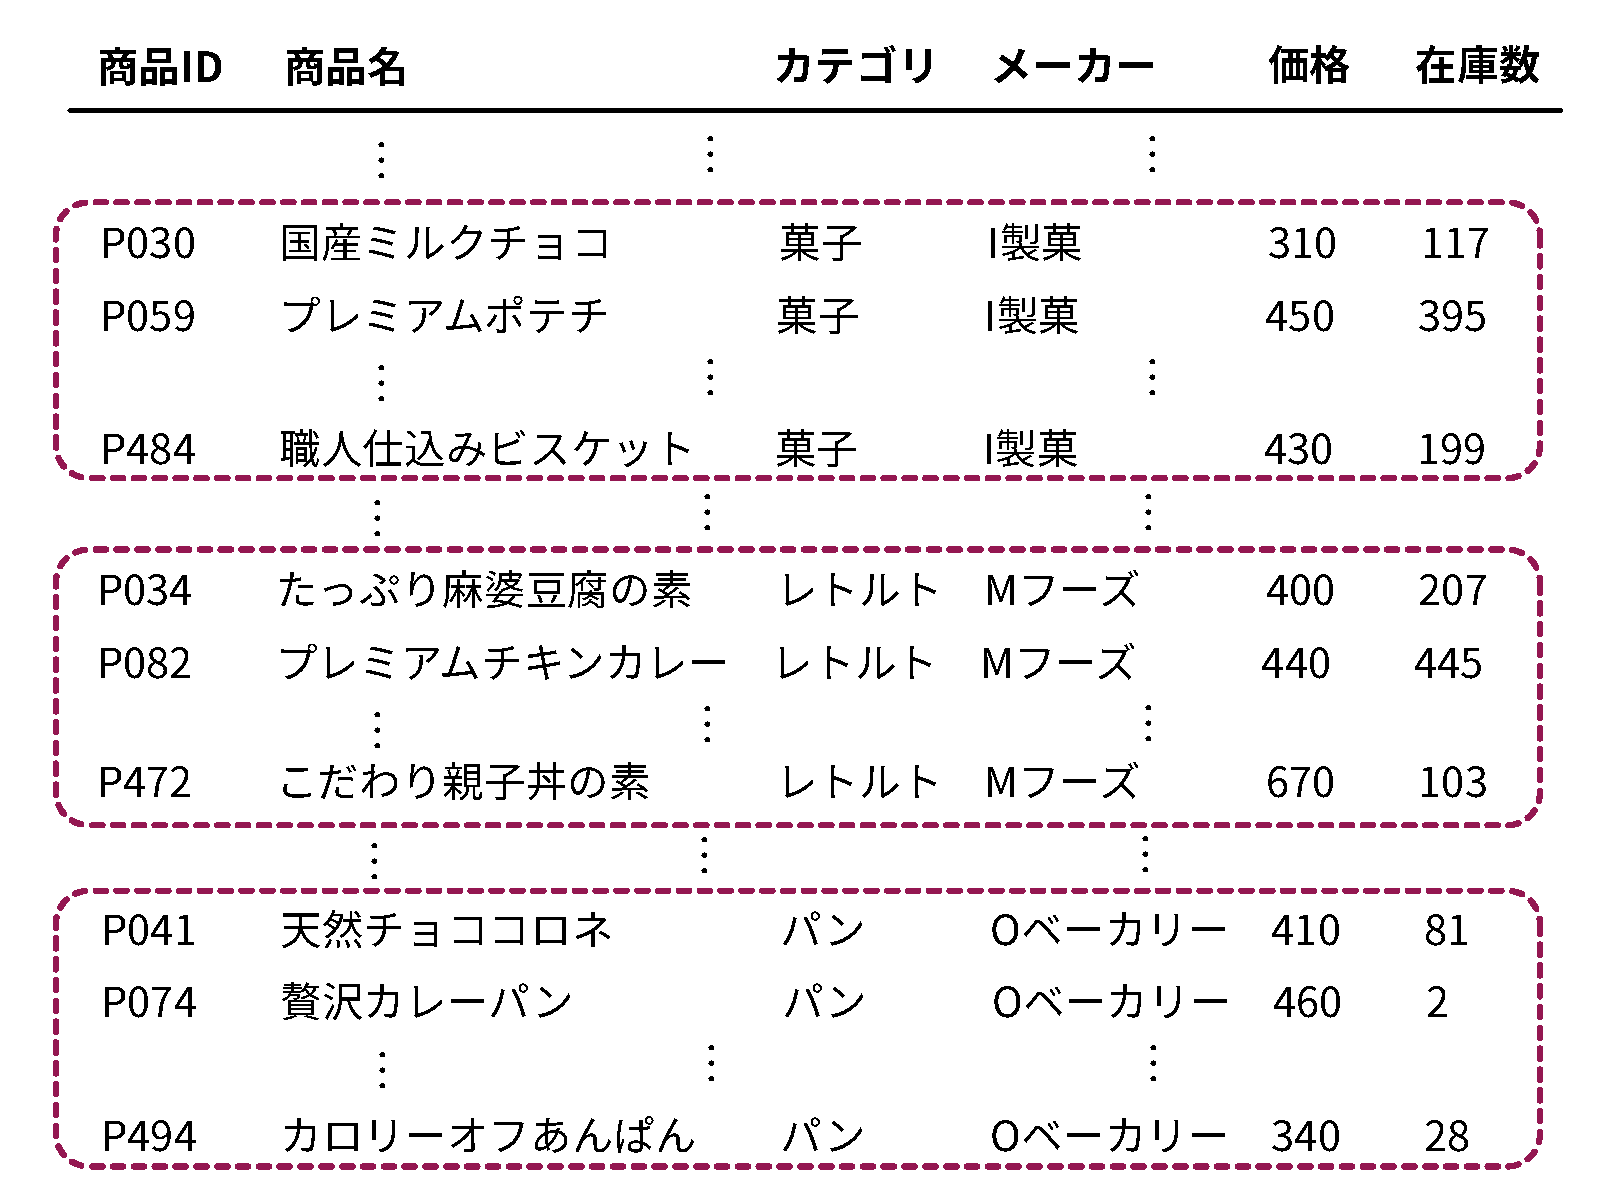
\includegraphics[width=0.95\textwidth]{figure/sql-part1/groupby.pdf}
    \caption{GROUP BY句によって「商品」テーブルを「メーカー」列の値でグループ化したイメージ図}
    \label{fig:groupby}
\end{figure}

コード\ref{code:sql-groupby}は，「商品」テーブルを用いて，「メーカー」ごとに商品の「在庫数」の平均値を計算するSQL文です．
このSQL文を実行すると，表\ref{tab:sql-groupby}のように，「商品」テーブルのレコードが「メーカー」列の値でグループ化され，グループごとに「在庫数」の平均値が計算されて表示されます．
メーカー名を表示させるために，\graybox{SELECT}句に「メーカー」列を指定していることに注意してください．
\begin{figure}[h]
    \begin{minted}[gobble=1,
        bgcolor=background,
        fontsize=\small,
        linenos=false]{sql}

    SELECT
        メーカー,
        AVG(在庫数) AS 平均在庫数 --- コメント: 列名を「平均在庫数」に変更
    FROM
        商品
    GROUP BY
        メーカー;

    \end{minted}
    \captionsetup{name=コード}
    \caption{「商品」テーブルを用いて，「メーカー」ごとに商品の「在庫数」の平均値を計算するSQL文}
    \label{code:sql-groupby}
\end{figure}
\begin{table}[h]
    \centering
    \caption{「商品」テーブルを用いて，「メーカー」ごとに商品の「在庫数」の平均値を計算した結果}
    \scalebox{0.93}{
    \begin{tabular}{@{}ll@{}}
    \toprule
    \textbf{メーカー} & \textbf{平均在庫数} \\ \midrule
A製パン & 255.8 \\
Bフーズ & 249.0 \\
C食品 & 265.3 \\
Dフード & 274.3 \\
E食品 & 285.1 \\
$\vdots$ & \\
Q醤油 & 246.3 \\
 \bottomrule
    \end{tabular}
    }
    \label{tab:sql-groupby}
\end{table}

\graybox{GROUP BY}句は\graybox{WHERE}句と組み合わせて使うこともできます．
\graybox{WHERE}句を使うことで，ある条件で絞り込んだレコード集合に対して\graybox{GROUP BY}を適用することができます．

コード\ref{code:sql-groupby-where}は，「商品」テーブルの中で価格が360円以上の商品が何件あるか，それら商品の平均価格はいくらかについて，メーカーごとに集計するSQL文です．
\graybox{WHERE}句を使うことで，集約対象を「価格が360円以上の商品レコード」に絞り込んだ後，グループ化と集約を行っていることに注意しましょう．
このSQL文を実行すると，表\ref{tab:sql-groupby-where}のような結果が得られます．
\begin{figure}[h]
    \begin{minted}[gobble=1,
        bgcolor=background,
        fontsize=\small,
        linenos=false]{sql}

    SELECT
        メーカー,
        COUNT(*) AS 商品数, --- コメント: 列名を「商品数」に変更
        AVG(価格) AS 平均価格 --- コメント: 列名を「平均価格」に変更
    FROM
        商品
    WHERE
        価格 >= 360
    GROUP BY
        メーカー;

    \end{minted}
    \captionsetup{name=コード}
    \caption{「商品」テーブルを用いて，価格が360円以上の商品の数と平均価格を「メーカー」ごとに集計するSQL文}
    \label{code:sql-groupby-where}
\end{figure}
\begin{table}[h]
    \centering
    \caption{「商品」テーブルを用いて，価格が360円以上の商品の数と平均価格を「メーカー」ごとに集計した結果}
    \scalebox{0.93}{
    \begin{tabular}{@{}lll@{}}
    \toprule
    \textbf{メーカー} & \textbf{商品数} & \textbf{平均価格} \\ \midrule
A製パン & 5 & 474.0 \\
Bフーズ & 11 & 432.7 \\
C食品 & 19 & 461.1 \\
Dフード & 35 & 674.3 \\
E食品 & 17 & 669.4 \\
& $\vdots$ & \\
Q醤油 & 25 & 707.6 \\
 \bottomrule
    \end{tabular}
    }
    \label{tab:sql-groupby-where}
\end{table}

上のケースでは集約前にレコードを絞り込んでいましたが，グループごとに集計した後に指定した条件を満たした結果を抽出したいケースもあります．
そのようなニーズに応えるのが\graybox{HAVING}句です．
\graybox{HAVING}句は\graybox{WHERE}句と同じ形式で条件を指定しますが，\graybox{GROUP BY}句の後に書くことに注意しましょう（\graybox{WHERE}句は\graybox{GROUP BY}句の前）．

コード\ref{code:sql-groupby-having}は，「商品」テーブルのレコードについて，「メーカー」ごとに取り扱っている商品数と商品の平均価格を集約し，その後商品の平均価格が360円以上のメーカーの情報だけを残して抽出するSQL文です．
実行結果は表\ref{tab:sql-groupby-having}のようになりますが，\graybox{WHERE}句を用いた場合と\graybox{HAVING}句を用いた場合で挙動が異なることを意識しましょう．
\begin{figure}[h]
    \begin{minted}[gobble=1,
        bgcolor=background,
        fontsize=\small,
        linenos=false]{sql}

    SELECT
        メーカー,
        COUNT(*) AS 商品数,
        AVG(価格) AS 平均価格
    FROM
        商品
    GROUP BY
        メーカー
    HAVING
        AVG(価格) >= 360; -- コメント: WHEREとは違って，HAVINGはGROUP BYの後に書く

    \end{minted}
    \captionsetup{name=コード}
    \caption{「商品」テーブルを用いて，価格が360円以上の商品の数と平均価格を「メーカー」ごとに集計した後，平均価格が360円以上のメーカーの情報だけを抽出するSQL文}
    \label{code:sql-groupby-having}
\end{figure}
\begin{table}[h]
    \centering
    \caption{「商品」テーブルを用いて，価格が360円以上の商品の数と平均価格を「メーカー」ごとに集計した後，平均価格が360円以上のメーカーの情報だけを抽出した結果}
    \scalebox{0.93}{
    \begin{tabular}{@{}lll@{}}
    \toprule
    \textbf{メーカー} & \textbf{商品数} & \textbf{平均価格} \\ \midrule
Dフード & 42 & 600.0 \\
E食品 & 22 & 573.6 \\
Fファーム & 68 & 459.9 \\
L食品 & 35 & 598.3 \\
Mフーズ & 15 & 480.7 \\
Q醤油 & 27 & 678.5 \\
 \bottomrule
    \end{tabular}
    }
    \label{tab:sql-groupby-having}
\end{table}

\begin{notebox}{SQLの処理順序（再び）}
本章では\graybox{SELECT}句，\graybox{FROM}句，\graybox{WHERE}句，\graybox{ORDER BY}句，\graybox{GROUP BY}句，\graybox{HAVING}句が登場しました．

関係データベース管理システムは，以下の順序でSQL文の評価と処理を行います．
\begin{enumerate}
\item \graybox{FROM}句で指定した表を参照
\item \graybox{WHERE}句があれば\graybox{WHERE}句で指定された条件を満たすレコードを選択．なければ\graybox{FROM}句で指定した表中の全レコードを選択．
\item （\graybox{GROUP BY}句があれば）ステップ2で選択されたレコードをグループ化する
\item （\graybox{HAVING}句があれば）ステップ3でまとめられたグループに対する条件付けを行う
\item 条件を満たしたものについて，\graybox{SELECT}句で指定された値を抽出する．
\item （\graybox{ORDER BY}句があれば）指定された基準に基づきレコードをソートする
\end{enumerate}

SQLは「何が欲しいか」を記述する宣言型の言語です．
料理に例えると，SQL文は料理のレシピと言えます．
まず冷蔵庫（\graybox{FROM}）から食材（テーブル）を出し，傷んだものを取り除き（\graybox{WHERE}），同じ種類の食材をまとめ（\graybox{GROUP BY}），お皿に盛り付けて（\graybox{SELECT}），最後に見栄え良く並べ替えます（\graybox{ORDER BY}）．
SQL文を書く際には，SQL文で書かれた内容がどのような順序で処理されるかを意識しましょう．
\end{notebox}


% ---------------------------------------
\section{クイズ}
% ---------------------------------------

本クイズでは，独立行政法人統計センターが公開している教育用標準データセット（SSDSE）の基本素材SSDSE-E\footnote{教育用標準データセット（SSDSE）: \url{https://www.nstac.go.jp/use/literacy/ssdse/\#SSDSE-E}}から，著者が抜粋・加工したデータを用います．
加工済みのデータのファイル（\graybox{SSDSE.db}）はコチラのURL（\url{https://xxxxxxx}）よりダウンロードできます．

ダウンロードしたファイル\graybox{SSDSE.db}はSQLite形式のデータベースファイルです．
本章の冒頭で説明したDB Browser for SQLiteなどのツールを用いてこのファイルを開くと，データベース内のテーブルを参照することができます．

\graybox{SSDSE.db}には複数のテーブルが格納されていますが，このクイズで用いるのは\graybox{population}テーブルです．
表\ref{tab:population-table}の通り，\graybox{population}テーブルには，47ある各都道府県に関する総人口，小学校児童数，中学校生徒数，高等学校生徒数，大学学生数のデータが2021年度，2020年度分格納されています．
\begin{table}[tb]
    \centering
    \caption{SSDSE-Eからクイズ用に著者が抜粋・加工したデータ: populationテーブル}
    \scalebox{0.73}{
    \begin{tabular}{@{}rrrrrrrr@{}}
    \toprule
    \textbf{地域コード} & \textbf{都道府県} & \textbf{調査年度} & \textbf{総人口} & \textbf{小学校児童数} & \textbf{中学校生徒数} & \textbf{高等学校生徒数} & \textbf{大学学生数} \\ \midrule
    R01000 & 北海道 & 2021 & 5183000 & 231714 & 122742 & 115335 & 79729 \\
    R02000 & 青森県 & 2021 & 1221000 & 54460  & 29940  & 30543  & 15419 \\
    R03000 & 岩手県 & 2021 & 1196000 & 55597  & 30269  & 29980  & 11340 \\
    R04000 & 宮城県 & 2021 & 2290000 & 112246 & 58748  & 55329  & 49580 \\
    R05000 & 秋田県 & 2021 & 945000  & 38992  & 21924  & 21448  & 8904  \\
    &        &      &          & $\vdots$  &        &        &       \\
    R46000 & 鹿児島県 & 2021 & 1576000  & 88636  & 45294  & 43029  & 15477  \\
    R47000 & 沖縄県  & 2021 & 1468000  & 101342 & 49716  & 43221  & 17882  \\
    R01000 & 北海道  & 2020 & 5224614  & 236396 & 123129 & 119773 & 79409 \\
           &        &      &          & $\vdots$  &        &        &       \\ \bottomrule
    \end{tabular}
    }
    \label{tab:population-table}
\end{table}

\graybox{population}テーブルを対象として，以下のSQL課題に取り組んでください．

\subsubsection{Q1. 射影}
「都道府県」「調査年度」「大学学生数」フィールドに限定して，\graybox{population}テーブルのレコードを表示するSQL文を書きなさい．
なお，表示するレコード数は30件としなさい．

\subsubsection{Q2. 選択 (1/3)}
\graybox{population}テーブル内のレコードのうち，都道府県が\graybox{愛知県}で調査年度が\graybox{2020}であるものを表示するSQL文を書きなさい．

\subsubsection{Q3. 選択 (2/3)}
\graybox{population}テーブル内のレコードのうち
\begin{itemize}
\item 総人口が\graybox{300万人}未満，かつ
\item 都道府県名が\graybox{県}で終わる，かつ
\item 中学校生徒数が高等学校生徒数以下
\end{itemize}
であるレコードを表示するSQL文を書きなさい．

\subsubsection{Q4. 選択 (3/3)}
Q3のSQL文を修正して，Q3の条件を満たす都道府県を表示するSQL文を書きなさい．
ただし，出力される都道府県名に重複がないようにしなさい．

\subsubsection{Q5. ソート (1/2)}
\graybox{population}テーブル内のレコードのうち調査年度が\graybox{2021}のものについて，大学学生数の大きいもの順に並び替えて表示するSQL文を書きなさい．

\subsubsection{Q6. ソート (2/2)}
\graybox{population}テーブル内のレコードのうち調査年度が\graybox{2021}のものについて，総人口に占める大学学生数の割合が大きいもの順に並び替えて表示するSQL文を書きなさい．
その際，総人口に占める大学学生数の割合も合わせて表示しなさい．

\subsubsection{Q7. GROUP BY (1/3)}
\graybox{population}テーブル内のレコードに対して都道府県ごとの集約演算を行い，都道府県別に
\begin{itemize}
\item （調査期間中の）大学学生数の平均
\item （調査期間中の）大学学生数の最大値と最小値の差
\end{itemize}
を求めるSQL文を書きなさい．

\subsubsection{Q8. GROUP BY (2/3)}
\graybox{population}テーブル内の総人口が\graybox{300万人}を超えるレコードに対して調査年度ごとの集約演算を行い，
調査年度別に
\begin{itemize}
\item 「（各地域コードにおける）小学校児童数と中学校生徒数の合計」の平均
\item「（各地域コードにおける）高等学校生徒数と大学学生数の差」の平均
\item「（各地域コードにおける）高等学校生徒数と大学学生数の差」の最小値
\item「（各地域コードにおける）高等学校生徒数と大学学生数の差」の最大値
\end{itemize}
を求めるSQL文を書きなさい．

\subsubsection{Q9. GROUP BY (3/3)}
\graybox{population}テーブルのレコードに対して都道府県ごとの集約演算を行い，
都道府県別に
\begin{itemize}
\item 「（調査期間中の）総人口」の平均
\item 「（調査期間中の）高等学校生徒数」の平均
\item 「（調査期間中の）大学学生数」の平均
\item 「（調査期間中の）高等学校生徒数と大学学生数の差」の平均
\end{itemize}
を求めるSQL文を書きなさい．
ただし，「（調査期間中の）大学学生数と高等学校生徒数の差」の平均が\graybox{10000}以下になるものだけを表示しなさい．

